\documentclass[11pt]{article}
\usepackage{enumitem}
\usepackage{amsmath,amsthm,amssymb}
\usepackage{color}
\usepackage{graphicx}
\graphicspath{ {./images/} }

\begin{document}
\date{} 
\title{Lab Report 1\\--\\\large CPE282 Fall 2020}
\author{Brennen Green}
\maketitle

\section{CMOS}
\subsection[]{Inverter:}
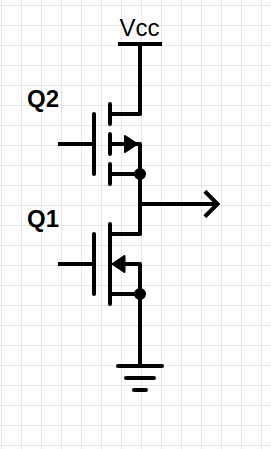
\includegraphics[width=4cm, keepaspectratio]{inverter}\newline
This implementation proved to be a learning experience. While my theoretical design
from the prelab was correct, I lacked some knowledge regarding the proper orientation
of the MOSFETs. Once I cleared up the issue, and properly oriented the
source and drains of the MOSFETs it worked like a charm.
\subsection[]{NAND:}
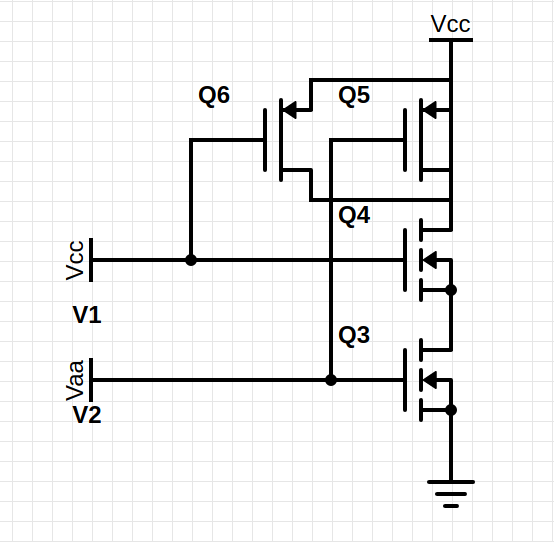
\includegraphics[width=4cm, keepaspectratio]{NAND}\newline
This implementation was rather smooth sailing, my implementation followed my design
from the prelab identically and worked first try.
\subsection[]{AND:}
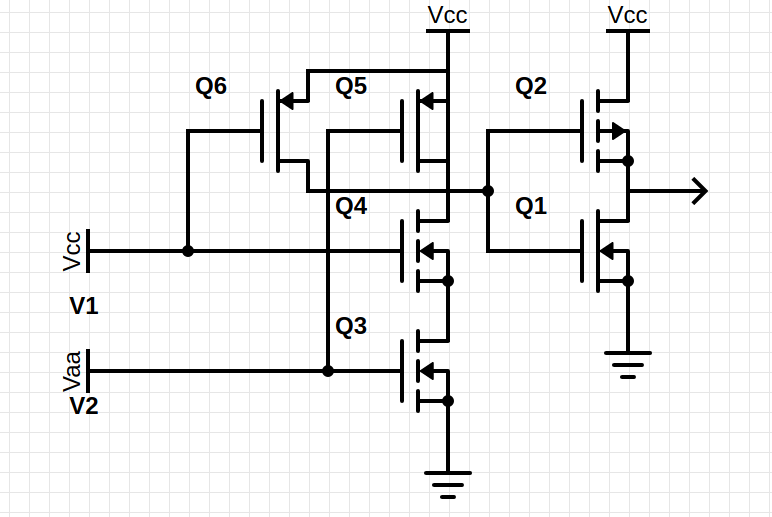
\includegraphics[width=6cm, keepaspectratio]{AND}\newline
There wasn't much to this implementation at all, just simply routed a new wire
from the output of my NAND to the input of my Inverter and we were good to go.
\newpage

\section{TTL}
\subsection[]{NAND:}
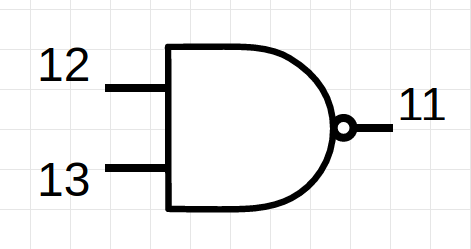
\includegraphics[width=4cm, keepaspectratio]{NAND-C}\newline
\subsection[]{AND:}
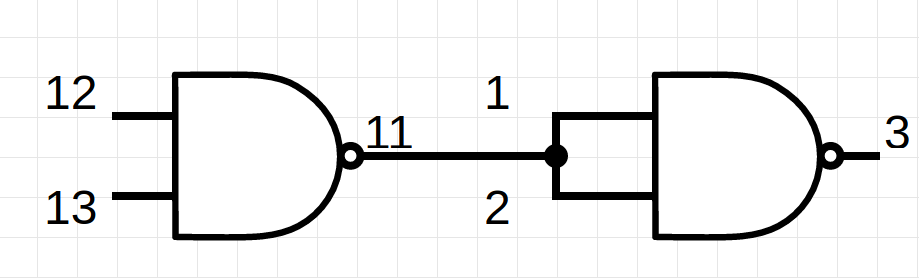
\includegraphics[width=4cm, keepaspectratio]{AND-C}\newline

It's worth grouping these two into one paragraph because they were very straight forward.
I followed my prelab to the T and it worked on the first try. The TTL's are really easy to 
work with.

\end{document}

